% Chapter 1

\chapter{Introduction} % Main chapter title

\label{Chap1} % For referencing the chapter elsewhere, use \ref{Chapter1} 

%----------------------------------------------------------------------------------------

% Define some commands to keep the formatting separated from the content 
\newcommand{\keyword}[1]{\textbf{#1}}
\newcommand{\tabhead}[1]{\textbf{#1}}
\newcommand{\code}[1]{\texttt{#1}}
\newcommand{\file}[1]{\texttt{\bfseries#1}}
\newcommand{\option}[1]{\texttt{\itshape#1}}

%----------------------------------------------------------------------------------------
Many of the natural phenomena taking place in this universe have made human beings to wonder what causes these phenomena. We, the human beings have been trying to find out if there is (or are) any fundamental principle(s) that are responsible for this. Based on today's understanding, there are four fundamental forces:
\begin{itemize}
\item Gravitational force: this causes apple to fall and also the planets to revolve around the sun.
\item Electromagnetic force: the one which holds atoms together, basic principle in chemistry and almost everything, except gravity, that we come across in daily life is governed by this force.
\item Weak force: $\beta$ decay taking place in the nucleus is because of this force.
\item Strong force: this force holds protons and neutrons together in the nucleus.
\end{itemize}
The matter that we see around us is made up of tiny particles, atoms. Atoms are made up of a nucleus (consisting of protons and neutrons, collectively called nucleons) and electrons. Nucleons have more fundamental particles called quarks. So the matter around us can be thought of as some combination of electrons and quarks. Apart from these, there are also other fundamental particles, some of which are similar to electrons and quarks but not the constituents of matter, some are mediators of the fundamental forces and one is responsible for the particles to have mass. Totally there are 18 such fundamental particles which we know today and four forces. Can we put all these particles and forces into a framework and try to understand the phenomena around us? The attempt that we made so far for this purpose has led to standard model (SM) of physics. Our attempt is not complete because in the framework of SM, we could not fit gravitational force or interaction and also the mediator of gravity, graviton. The graviton is a hypothetical particle, not experimentally detected, is not included in the SM. So the SM consists of 17 fundamental particles and 3 fundamental forces.

The SM has successfully explained many of the experimental results with very high degree of precision. But the SM is not a complete story of the universe, one of the simple reason being, not having gravity included in it. There are many other issues in the SM, such as the inability to explain dark matter and dark energy in the universe, matter anti-matter asymmetry etc, and many theoretical problems. To address many of the issues in the SM, many extensions of SM have been proposed, one of them being the supersymmetry (SUSY). SUSY predicts that for every SM particle, there is a superpartner similar in all the quantum numbers and properties except that the spin quantum number differs by half a unit. Failure to observe SUSY particles with same mass as SM particles (we did not find an SUSY electron, called selectron or sproton, sneutron etc), led to the ideas of breaking of this symmetry. There are many ways of breaking SUSY, one of them being gauge mediated SUSY breaking (GMSB). In scenarios with GMSB, gravitino (super partner of hypothetical graviton) is the lightest SUSY particle (LSP) and it is stable. \textcolor{red}{The stability of LSP is a requirement from R-parity conservation which does not allow SUSY particle decay into only SM particles.} LSP is weakly interacting particle and hence it's detection is very difficult in an experiment.

The compact muon solenoid (CMS) detector at the large hadron collider (LHC), CERN has a lot of potentials for testing the SM and also to carry out searches for beyond SM particles, such as SUSY particles. At the LHC, proton-proton collisions take place at the center of mass energy of 13 TeV. SUSY particles can be produced in these collisions if they exist and accessible at the LHC. In GMSB models, events with photon, quarks of light or bottom flavor and missing transverse momentum are expected. Missing transverse momentum is the signature of weakly interacting LSPs in the detector.

This thesis is about a SUSY search with at least one photon, light or bottom flavor jets which originate from quarks and large missing transverse momentum using the data collected in the year 2016 at the CMS detector. This chapter \ref{Chap1} gives a very brief introduction to SM, its limitations and supersymmetric extensions of SM and GMSB models. Chapter \ref{Chap2} describes the experimental set up consisting of LHC and the CMS detector. My work on hadron forward calorimeter of CMS is also described in this chapter.  The main analysis is discussed in \ref{Chap3}. Summary and some possible searches in the future is described in the final chapter \ref{Chap4}.


\section{Standard model particles}
The SM of particle physics consists of 3 generations of quarks and leptons (Table \ref{tab:SM}), gauge bosons which are mediators of strong, electromagnetic (EM) and weak force, and a scalar higgs boson (Table \ref{tab:SM_boson}).

\begin{table}[h!]
\centering
\caption{Leptons and quarks of SM with their properties}
\label{tab:SM}
\begin{tabular}{c|c|c|c|c|c}
\hline
\multicolumn{6}{c}{Leptons (spin $\frac{1}{2}$)}\\ \hline
Gen.         & Particle & Charge & Mass (MeV) & Interactions\footnotemark & \textcolor{red}{Chiral state}\\ \hline
%				   &		  &		   &            &               &\\ \hline
\multirow{2}{*}{1} & $\nu_e$  &  0     & $<2\times10^{-6}$     & Weak & \multirow{2}{*}{$\begin{bmatrix} \nu_e \\ e_{L}\end{bmatrix},\ e_{R}$}\\
& $e$      &	 $\mp1$ & 0.511  & EM, Weak      &	\\ \hline
\multirow{2}{*}{2} & $\nu_\mu$  &  0     & $<0.19$  & Weak & \multirow{2}{*}{$\begin{bmatrix} \nu_\mu \\ \mu_{L}\end{bmatrix},\ \mu_{R}$}\\
& $\mu$      &	 $\mp1$ & 105.7  & EM, Weak      &	\\ \hline
\multirow{2}{*}{3} & $\nu_\tau$  &  0     & $<18.2$  & Weak & \multirow{2}{*}{$\begin{bmatrix} \nu_\tau \\ \tau_{L}\end{bmatrix},\ \tau_{R}$}\\
& $\tau$      &	 $\mp1$ & 1777  & EM, Weak      &	\\ \hline

\multicolumn{6}{c}{Quarks (spin $\frac{1}{2}$)}\\ \hline
Gen.        & Particle & Charge & Mass (MeV) & Interactions & \textcolor{red}{Chiral state}\\ \hline
\multirow{2}{*}{1} & $u$  &  $\pm\frac{2}{3}$     & $\approx 2.2$     & \multirow{6}{*}{Strong, EM, \newline Weak} & \multirow{2}{*}{$\begin{bmatrix} u_L \\ d_{L}\end{bmatrix},\ u_{R},\ d_R$}\\
 & $d$      &	 $\mp\frac{1}{3}$ & $\approx4.7$  &       &	\\ \cline{1-4} \cline{6-6}
\multirow{2}{*}{2} & $c$  &  $\pm\frac{2}{3}$     & $1.275\times10^{3}$     &  & \multirow{2}{*}{$\begin{bmatrix} c_L \\ s_{L}\end{bmatrix},\ c_{R},\ s_R$}\\
 & $s$      &	 $\mp\frac{1}{3}$ & $\approx95$  &       &	\\ \cline{1-4} \cline{6-6}
\multirow{2}{*}{3} & $t$  &  $\pm\frac{2}{3}$     & $173.1\times10^{3}$     &  & \multirow{2}{*}{$\begin{bmatrix} t_L \\ b_{L}\end{bmatrix},\ t_{R},\ b_R$}\\
 & $b$      &	 $\mp\frac{1}{3}$ & $\approx4.18\times10^{3}$  &       &	\\ \hline
\end{tabular}
\end{table}
\footnotetext{All particles with non-zero mass have gravitational interactions. But gravity is not a part of SM.}

\begin{table}[h!]
\centering
\caption{Gauge bosons and higgs boson in SM with their properties}
\label{tab:SM_boson}
\begin{tabular}{c|c|c|c|c|c}
\hline
Particle	&	Charge	&	Mass (GeV)	&	Spin	&	Force mediation	&	Mixing fields\\\hline
g			&	0		&	0			&	1		&	Strong			&	g\\
$\gamma$	&	0		&	0			&	1		&	EM				&	$W_3,B$\\
\ce{W}			&	$\mp1$	&	80.4		&	1		&	Weak			&	$W_1,W_2$\\
\ce{Z}			&	0		&	91.2		&	1		&	Weak			&	$W_3,B$\\
\ce{H}			&	0		&	125.2		&	0		&	-				&	$H_u,H_d$\\\hline
\end{tabular}
\end{table}
Categorization of the quarks and leptons into 3 generations is done based on their masses~\cite{PhysRevD.98.030001} and properties. First generation consists of lightest and the third generation consists of heaviest particles. Neutrinos are grouped according to their interactions and their exact masses are unknown. The masses of SM particles are not predicted by the theory, but they are measured quantities in experiments. All the charged (in this thesis charge always refers to electric charge) particles have EM interactions. Neutral leptons, neutrinos, have only weak interactions. Quarks have additional quantum number, color, which is responsible for strong interaction. 

\section{Conservation laws and symmetry}
Experiments have played a significant role in development of the SM. Various observations from them lead to framing many laws of nature. Similar to the law of conservation of energy and momentum in basic physics, there are other laws of conservation such as charge, angular momentum, color charge, lepton number within each generation etc. Whenever there is a conservation law, then there is a symmetry associated with it and a symmetry also implies a conservation law. This relation between conservation law and symmetry is given by Noether's theorem~\cite{Noether1918}. Conservation of energy, linear momentum and angular momentum are connected with symmetry in time translation, space translation and rotation respectively. Gauge transformation invariance in electrodynamics lead to conservation of charge. These symmetries can be represented mathematically using symmetry groups. For example, group representing rotational symmetry is $SO(3)$. 

\section{Strong interactions}
The strong interaction is mediated by gluon and the theory is described by quantum chromodynamics (QCD). QCD is based on the symmetry group $SU(3)_C$, where $C$ represents color (red, green or blue), having 3 degrees of freedom and 8 generators or 8 gluon fields. The eight colors of gluon are:
\begin{equation*}
R\bar{G},\ R\bar{B},\ G\bar{R},\ G\bar{B},\ B\bar{R},\ B\bar{G},\ \frac{1}{\sqrt{2}}(R\bar{R}-G\bar{G}),\ \frac{1}{\sqrt{6}}(R\bar{R}+G\bar{G}-2B\bar{B}) 
\end{equation*}
$SU(3)_C$ is a non-abelian gauge group which means that the gluons have self interactions. Quarks carry one color charge (red green or blue) and gluons are bi-colored having one of the 8 colors mentioned above. All the observed hadrons and mesons are colorless, in other words, no isolated quarks or gluons exist. The strength of strong interaction increases with distance (or decreases with energy). At very large energy, strong interaction becomes very small and this behavior is named as asymptotic freedom \cite{PhysRevLett.30.1343}\cite{PhysRevLett.30.1346}. As two quarks are separated from each other, quark-antiquark pair are created making initial quarks no longer isolated.

\section{Electro-weak interactions}
The interaction between charged particles is described by quantum electrodynamics (QED) which is based on the symmetry group $U(1)$. The mediator of this interaction is massless spin 1 photon. Unlike QCD, there are no self interactions of the force mediator since photon does not carry any charge.

The neutral leptons, neutrinos, take part only in weak interactions whose description is based on $SU(2)_L$ symmetry. The mediators of this force are massive W and Z bosons. All the leptons and quarks of SM have weak interactions and neutrinos have only weak interaction. Weak theory is a chiral theory which implies that only left handed particles or right handed antiparticles participate in the interactions. A consequence of chiral theory is that there is no place for right handed neutrinos or left handed anti-neutrinos within SM. In weak interactions, some of the quantum numbers which are conserved in strong and EM interactions, need not be conserved, namely: parity (P), charge conjugation (C) and time reversal (T).

At high energy, weak and EM interactions become indistinguishable and those interactions are described by electro-weak (EW) theory \cite{PhysRevLett.19.1264}\cite{Salam1959}\cite{Glashow:1959wxa} which obeys $SU(2)\otimes U(1)$ symmetry. Since the force mediators are spin-1 bosons, the theory must obey gauge invariance. Based on the gauge principle, it is concluded that the observed $\gamma, W^\pm$ and Z are mixtures of $W_1,\ W_2,\ W_3,$ and $B$ fields,
\begin{align}
W^\pm & = (W_1 \mp iW_2)/\sqrt{2}\\
Z & = -B\sin\theta_W + W_3\cos\theta_W\\
\gamma &= B\cos\theta_W + W_3\sin\theta_W
\end{align}
where $\theta_W$ is called the weak mixing angle and $B$ is such that its predictions are consistent with properties of $\gamma$ \cite{MartinShaw}.

\section{The Higgs mechanism}
Local gauge invariance demands force mediators to be massless. Indeed, this is the case for QCD and QED in which gluon and photon are massless. But the weak force mediators $W^\pm$ and $Z$ bosons are observed to be massive and were discovered at CERN in 1983 \cite{ARNISON1983103}\cite{BANNER1983476}\cite{1983398}\cite{BAGNAIA1983130}. A spontaneous symmetry breaking mechanism was proposed by Englert, Brout and Higgs \cite{Higgs:1964pj}\cite{Englert:1964et} by which the gauge bosons can acquire mass through the interaction with a new scalar filed, called Higgs field. The vacuum expectation value of the Higgs field is nonzero and when the gauge bosons interact with such a field the theory is not invariant under gauge transformations and the gauge bosons become massive. The ratio of masses of $W^\pm$ and $Z$ boson is given by
\begin{equation}
M_W/M_Z = \cos \theta_W
\end{equation}
The theory predicts a spin 0 quanta (particle) associated with the Higgs field. This particle was discovered at CERN by ATLAS and CMS experiments in 2012 \cite{Aad:2012tfa}\cite{Chatrchyan:2012xdj} and its mass was found to be $\approx 125$ \gev. The masses of quarks and leptons would have been zero, if there was no Higgs boson. If the interaction of particle is stronger with Higgs field, then its mass is expected to be higher. Top quark is the highest mass particle in SM and its coupling to Higgs is strongest. The interaction term between fermions and \higgs filed is given by $\mathcal{L}_{Yukawa} = - \lambda_f \bar{\psi}\textbf{H}\psi$ where $\psi$ is the Dirac field of the fermion, \textbf{\higgs} is the Higgs field and $\lambda_f$ is Yukawa coupling.

\section{Limitations of SM}
\label{SMLimitations}
With the discovery of the Higgs (H) boson, the SM is a complete theory which describes many of the experimental observations. The expectations from the SM agree with the experimental observations and Fig.\ref{fig:SigmaNew_v0} shows production cross sections for various SM processes and the measurements by the CMS experiment.
\begin{figure*}[h]
\centering
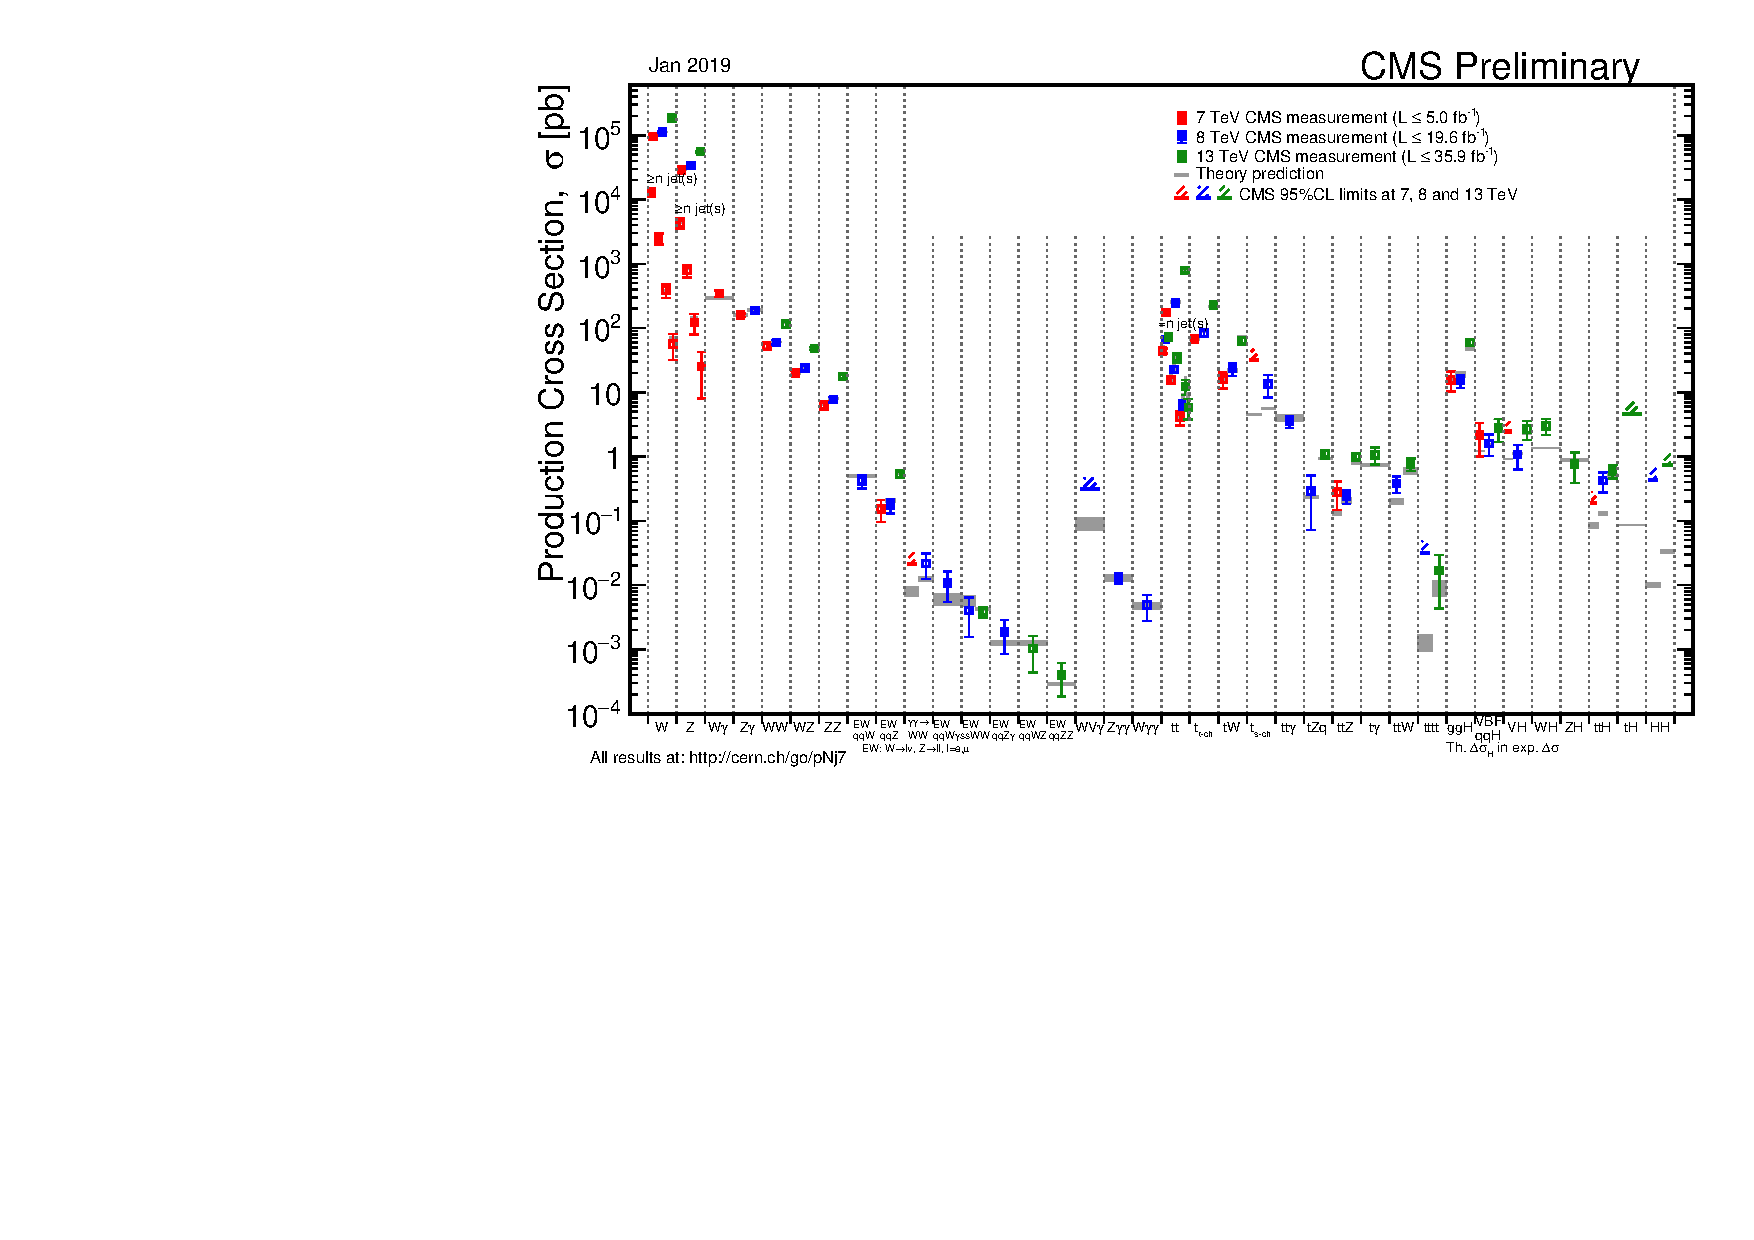
\includegraphics[width=0.9\linewidth]{../Figures/SigmaNew_v0}
\caption[SM cross section measurements by CMS]{Summary of the cross section measurements of SM processes by CMS experiment \cite{SMxsec}.}
\label{fig:SigmaNew_v0}
\end{figure*}
Although H was the last piece in the SM puzzle and we have discovered it, we are many theoretical issues and experimental results which are not explained by SM. From the theoretical point of view, observed mass of H at 125 \gev itself is an issue and it is called as hierarchy problem which will be discussed later. Some of the unsolved problems within SM framework are:
\begin{itemize}
\item Gravitational interactions cannot be explained by SM.
\item Matter-antimatter asymmetry: We do not understand why we see more matter in the universe than antimatter today. At the early stages of universe, both of these must have been created in equal amount. There must be a mechanism by which matter started to dominate over antimatter.
\item In SM masses of neutrinos is zero, whereas neutrino oscillations indicate that they have nonzero mass.
\item The universe comprises of 71.4\% of dark energy, 24\% of dark matter and only 4.6\% is ordinary matter that we know. What is explained by SM is less than 5\% of total universe content.
\item The strong, EM and weak gauge couplings are functions of energy scale. When these couplings are extrapolated to high energy, we expect all of them to unify at one energy. But this unification does not take place at one point within SM.
\item The \higgs boson gets corrections to its mass by loop diagram contributions, the largest contribution coming from top quark loop diagram (Fig.\ref{fig:hierarchy_problem_higgs}). This contribution is given by
\begin{equation}
\Delta m_{H}^2 = -\frac{|\lambda_t|^2}{8\pi^2}[\Lambda_{UV}^2 + \dots]
\label{eqn:HmassCorr}
\end{equation}
where $\lambda_t$ is the top Yukawa coupling ($\sim 1$) and $\Lambda_{UV}$ is the ultraviolet cutoff scale above which SM is not valid and its value is close to GUT (grand unified theory) scale, $10^{16}\gev$ or Planck scale, $> 10^{19}\ \gev$. With these large corrections, the mass of \higgs would have been $> 10^{16}\ \gev$ and not near 125 \gev. This is called hierarchy problem in SM.
\begin{figure}[h!]
\centering
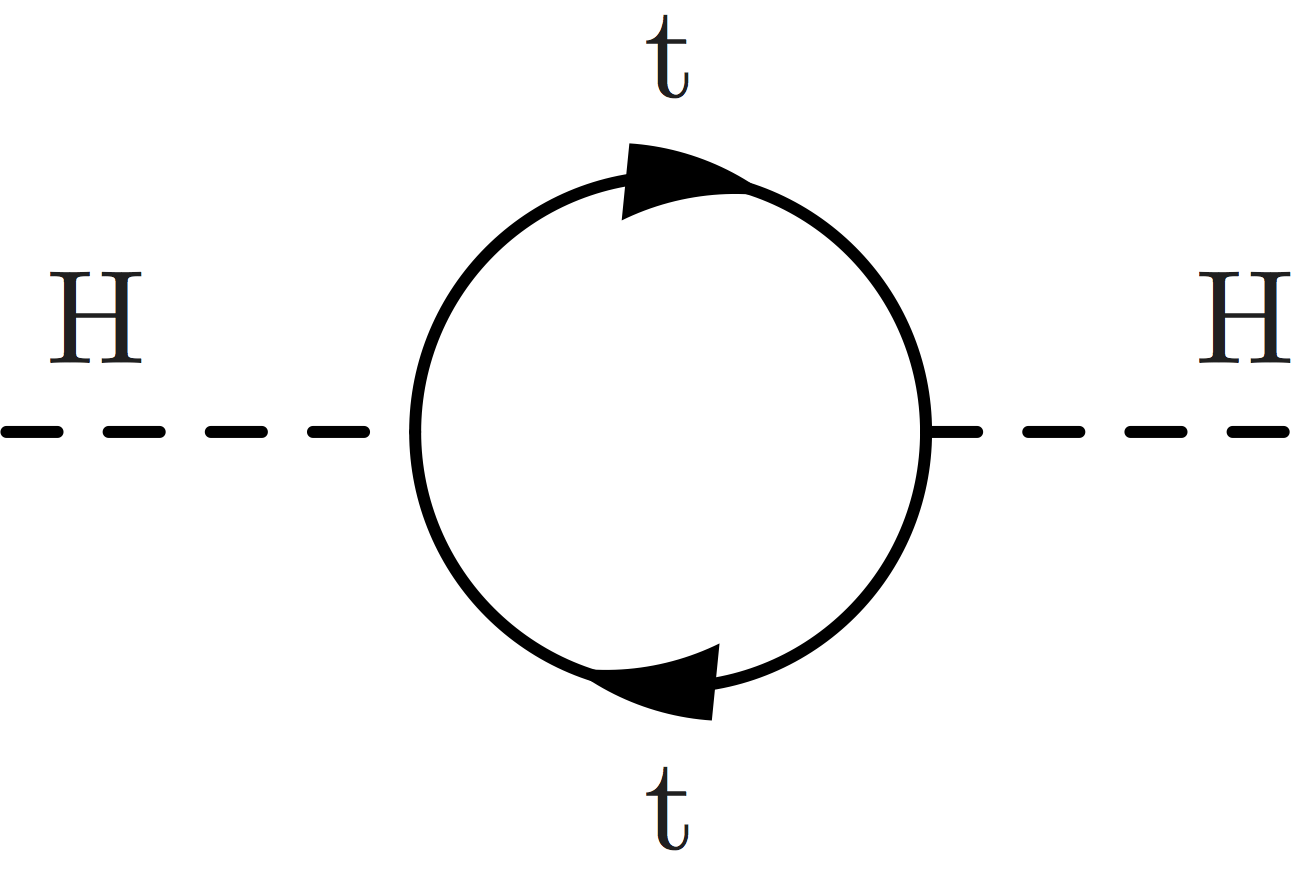
\includegraphics[width=0.35\linewidth]{../Figures/hierarchy_problem_higgs.png}
\caption{Top loop diagram contribution to \higgs mass}
\label{fig:hierarchy_problem_higgs}
\end{figure}
\end{itemize}

\section{Supersymmetric extension of SM}
To overcome the limitations of SM mentioned in Sec.\ref{SMLimitations}, we need extensions to SM which can address all (or some) of these issues without contradicting existing observations. One such extension is supersymmetry (SUSY) which can address last three issues mentioned above, namely the dark matter problem, gauge coupling unification and hierarchy problem.

To tackle hierarchy problem, if we can introduce a new term in eqn.\ref{eqn:HmassCorr} with similar correction but opposite sign, we might be able to get \higgs mass around 125 \gev. Naively speaking, what SUSY does is exactly this - it introduces a scalar partner for every SM fermion and a fermionic partner for bosonic SM particle and hence the corrections from superpartner loop diagrams cancel the corrections from SM particles. Superpartners of SM particles differ in spin by half a unit. For example, superpartner of top quark is top \textbf{s}quark(or \textbf{s}top) with spin 0. The superpartners of bosons have spin 1/2 and they are named with suffix \textit{ino}, such as gluino, photino etc. Fig.\ref{fig:hierarchy_problem_higgs_mass_stop} shows the contributions to \higgs mass from top loop and stop loop. The contribution from second loop diagram is given by eqn.\ref{eqn:HmassCorrSUSY} which has similar form as eqn.\ref{eqn:HmassCorr} but with an opposite sign.
\begin{figure*}[h!]
\centering
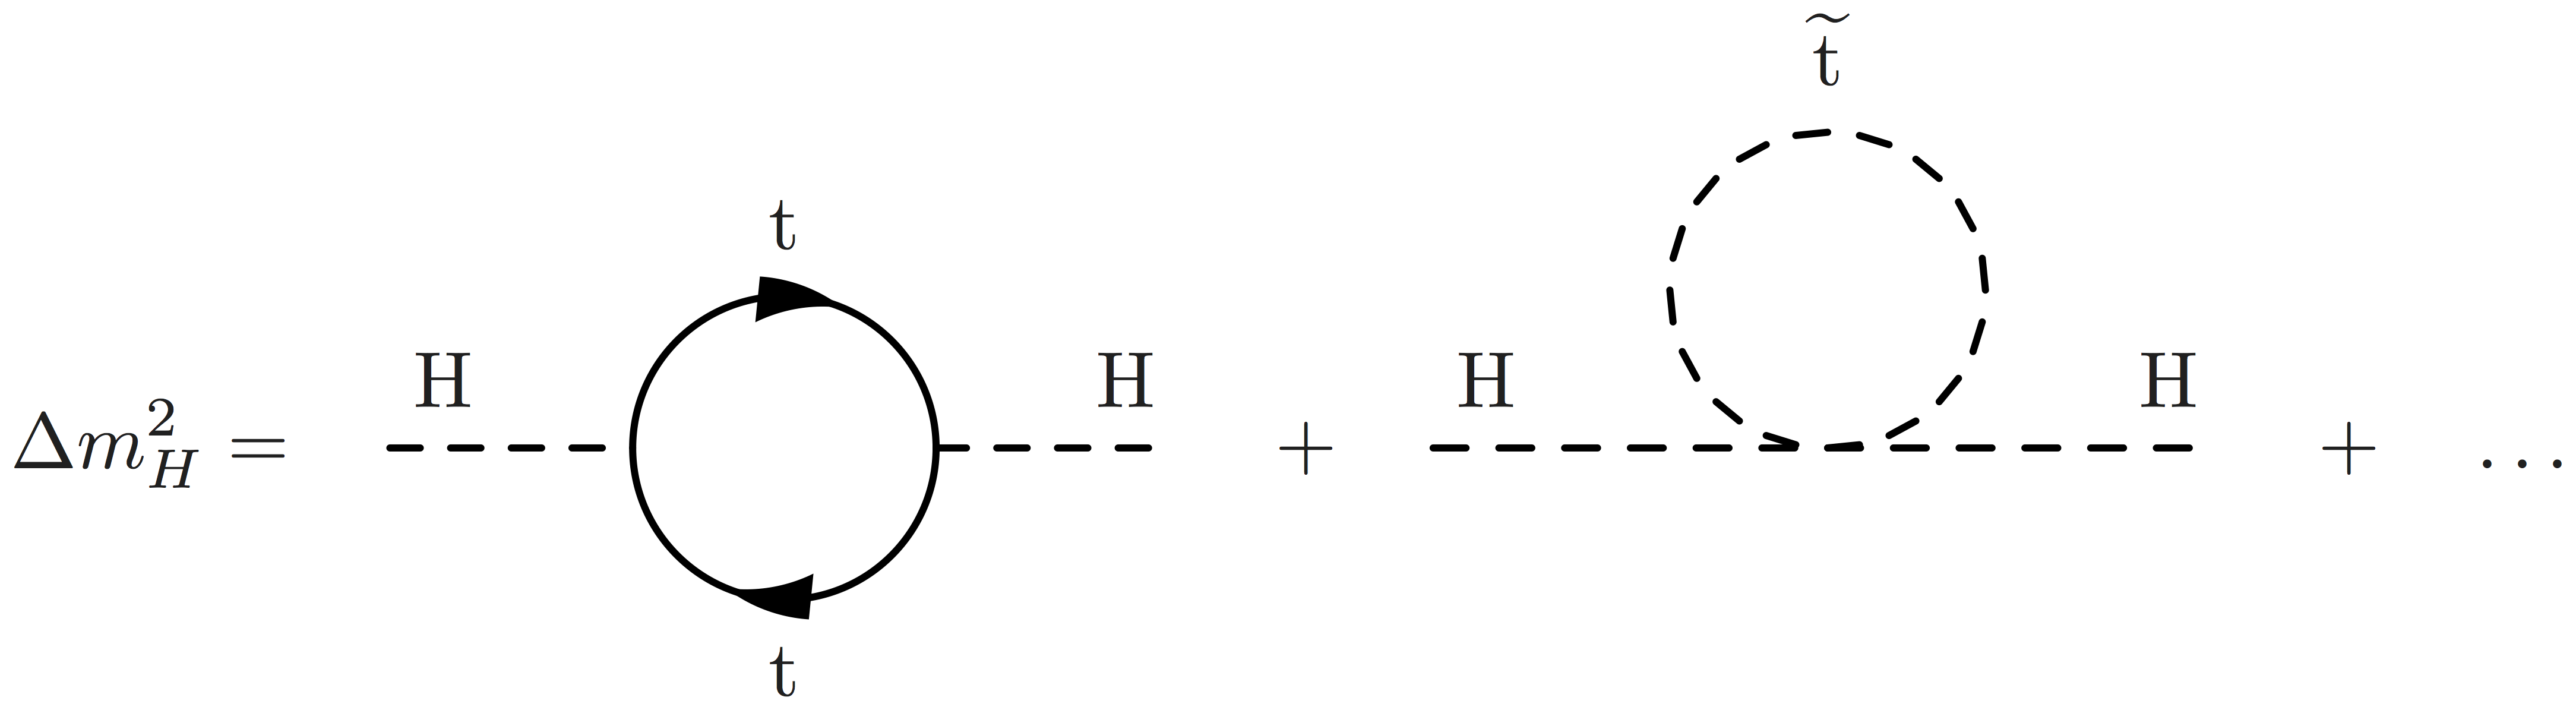
\includegraphics[width=0.8\linewidth]{../Figures/hierarchy_problem_higgs_mass_stop}
\caption{Corrections to \higgs mass from top loop and stop loop.}
\label{fig:hierarchy_problem_higgs_mass_stop}
\end{figure*}
\begin{equation}
(\Delta m_{H}^2)_{\text{SUSY}} = \frac{|\lambda_{\tilde{t}}|^2}{8\pi^2}[\Lambda_{UV}^2 + \dots]
\label{eqn:HmassCorrSUSY}
\end{equation}

We are interested in minimal supersymmetric extension of SM (MSSM) which is direct supersymmetrization of SM and has minimum number of new particle states and interactions consistent with phenomenology \cite{baer_tata_2006}. Table \ref{tab:SUSY} shows fields corresponding to various particles in the MSSM. These superpartners listed are not necessarily the mass eigen states of the theory because there can be mixing of gauginos and higgsinos \cite{Martin:1997ns}. The observable mass eigen states are charginos or neutralinos, denoted by $\tilde{\chi}^{\pm,0}$ and gluino which is not a mixture. Gauge and mass eigen states in MSSM are listed in table \ref{tab:SUSY2}.

\begin{table}[h!]
\centering
\caption[Chiral and gauge supermultiplets of MSSM]{Chiral supermultiplets and gauge supermultiplets in the MSSM \cite{Martin:1997ns}}
\label{tab:SUSY}
\begin{tabular}{|c|c|c|}
\hline   & spin 0  & spin 1/2  \\ 
\hline  
\multirow{3}{*}{squarks, quarks (x3 families)} & ($\tilde{u}_L\ \tilde{d}_L$) & (${u_L}\ {d_L}$) \\ 
								               & $\tilde{u}_R$				& $u_R$\\
                      						   & $\tilde{d}_R$				& $d_R$\\ \hline
\multirow{2}{*}{sleptons, leptons (x3 families)} & ($\tilde{\nu}\ \tilde{e}_L$) & (${\nu}\ {e_L}$) \\ 
                      						   & $\tilde{e}_R$				& $e_R$\\ \hline
\multirow{2}{*}{Higgs, higgsinos}			   & $(H^{+}_u\ H^{0}_u)$       & $(\tilde{H}^{+}_u\ \tilde{H}^{0}_u)$\\
											   & $(H^{0}_d\ H^{-}_d)$       & $(\tilde{H}^{0}_d\ \tilde{H}^{-}_d)$\\ \hline
                      						   & spin 1/2					& spin 1 \\ \hline
                  		gluino, gluon		   & $\tilde{g}$				& $g$ \\
                  		winos, W bosons		   & $\tilde{W}^\pm\ \tilde{W}^0$ & $W^\pm\ W^0$ \\
                  		bino, B boson		   & $\tilde{B}^0$				& $B^0$\\ \hline
\end{tabular} 
\end{table}

\begin{table}[h!]
\centering
\caption[Gauge and mass eigen states of MSSM]{Gauge and mass eigen states of MSSM \cite{Martin:1997ns}\cite{Rizzi:2646377}}
\label{tab:SUSY2}
\begin{tabular}{c|c|c|c}
\hline
Names	 					&	Spin			&	Gauge eigen states				&	Mass eigen states \\\hline
\multirow{3}{*}{squarks}	& \multirow{3}{*}{0}&	\susyP{u}$_L$ \susyP{u}$_R$ \susyP{d}$_L$ \susyP{d}$_R$ & same \\
							&					&	\susyP{c}$_L$ \susyP{c}$_R$ \susyP{s}$_L$ \susyP{s}$_R$ & same \\
							&					&	\susyP{t}$_L$ \susyP{t}$_R$ \susyP{b}$_L$ \susyP{b}$_R$ & \susyP{t}$_1$ \susyP{t}$_2$ \susyP{b}$_1$ \susyP{b}$_2$ \\\hline
\multirow{3}{*}{sleptons}	& \multirow{3}{*}{0}&	\susyP{e}$_L$ \susyP{e}$_R$ \susyP{\nu}$_e$ 			 & same \\
							&					&	\susyP{\mu}$_L$ \susyP{\mu}$_R$ \susyP{\nu}$_\mu$		 & same \\
							&					&	\susyP{\tau}$_L$ \susyP{\tau}$_R$ \susyP{\nu}$_\tau$	 &\susyP{\tau}$_1$ \susyP{\tau}$_2$ \susyP{\nu}$_\tau$ \\\hline
neutralinos & 1/2 & \susyP{B}$^0$ \susyP{W}$^0$ \susyP{H}$^{0}_{u}$ \susyP{H}$^{0}_{d}$ & \susyP{\chi}$^{0}_1$ \susyP{\chi}$^{0}_2$ \susyP{\chi}$^{0}_3$ \susyP{\chi}$^{0}_4$ \\\hline
charginos & 1/2 & \susyP{W}$^\pm$  \susyP{H}$^{+}_{u}$  \susyP{H}$^{-}_{d}$ & \susyP{\chi}$^{\pm}_1$ \susyP{\chi}$^{\pm}_2$ \\\hline
gluino 						&	1/2				&	\susyP{g}				&	same \\\hline
Higgs bosons				&	0				& \susyP{H}$^{0}_{u}$ \susyP{H}$^{0}_{d}$ \susyP{H}$^{+}_{u}$  \susyP{H}$^{-}_{d}$ & $h^0$ \higgs$^0$ $A^0$ $H^\pm$ \\\hline
gravitino	&	3/2	&	\grav	& same \\\hline
\end{tabular}
\end{table}

Since we have not observed SUSY particles at the same mass SM counterparts, SUSY is a broken symmetry and the masses of sparticles are larger than SM partners. The effective Lagrangian can be written as
\begin{equation}
\label{eqn:Lsusy}
\mathcal{L} = \mathcal{L_{\text{SUSY}}} + \mathcal{L_\text{{soft}}}
\end{equation}
The first term on RHS of eqn.\ref{eqn:Lsusy} preserves SUSY and contains gauge and Yukawa interactions. The second term breaks SUSY and contains mass terms and coupling parameters which should vanish at very high mass scale at which SUSY is unbroken. There are multiple ways to break SUSY and some of the popular ways are, gravity mediated or Planck scale mediated SUSY breaking (PMSB), anomaly mediated SUSY braking (AMSB) and gauge mediated SUSY breaking (GMSB). A brief discussion on GMSB is given in section \ref{sec:gmsb} to motivate the search for SUSY with photon which is the topic of this thesis.

\subsection{R-parity}
A multiplicative quantum number called \textit{R-parity} is introduced for every particle and sparticle to account for very strong experimental bounds on proton lifetime. The proton lifetime is $>10^{33}$ years \cite{PhysRevLett.102.141801} which is larger than the age of the universe. R-parity is defined as
\begin{equation}
\label{eqn:rparity}
P_R = (-1)^{3(B-L)+2s}
\end{equation}
where s is the spin, B and L are baryon number and lepton number respectively. All SM particles have even R-parity, $P_R=+1$ and SUSY particles have odd R-parity, $P_R=-1$. The important consequences of this parity conservation are:
\begin{itemize}
\item SUSY particles are always produced in pairs and any SUSY particle decay should involve even number of them. In other words, at any vertex, there should be even number of SUSY particles.
\item Lightest supersymmetric particle (LSP) must be stable. If LSP is neutral, then it could serve as dark matter candidate and account for 24\% of the universe content \cite{ELLIS1984453}, thereby solving one of the problems in SM.
\item All the non-LSP SUSY particle decay chains must result in odd number (usually 1) of LSPs.
\end{itemize}

\section{Gauge mediated SUSY breaking}
\label{sec:gmsb}
In GMSB scenarios \cite{Dine:1993yw,Dine:1994vc,Dine:1995ag,Meade:2008wd,Giudice:1998bp,Grajek:2013ola}, the communication between hidden sector, where SUSY breaking takes place, and the visible MSSM sector (consisting of chiral supermultiplets shown in table \ref{tab:SUSY2}) is via the ordinary gauge interactions. In comparison with other SUSY breaking scenarios, flavor changing processes and new sources of CP violation are naturally suppressed \cite{Dine:1993yw} in GMSB. The messengers communicating between MSSM and hidden sector also have $SU(3)_C \otimes SU(2)_L \otimes U(1)_Y$ interactions. The soft terms in MSSM come from loop diagrams involving these messengers, whose value is given by
\begin{equation}
m_{soft} \sim \frac{\alpha_{a}}{4\pi} \frac{\langle F \rangle}{M_{mess}}
\end{equation}
where $\alpha_{a}/{4\pi}$ is loop factor for Feynman diagrams involving gauge interactions, $F$ relates to the SUSY breaking scale and $M_{mess}$ is the messenger mass scale \cite{Martin:1997ns}.

GMSB permits a significantly lower symmetry-breaking scale ($\langle F\rangle$) than, e.g., gravity mediation, and therefore generically predicts that the gravitino (\grav) is the LSP~\cite{Meade:2008wd,PhysRevLett.38.1433,CREMMER1978231} whose value is given by
\begin{equation}
\label{massGrav}
m_{\grav}  \sim \ \langle F \rangle/M_P \sim \mathrm{keV}
\end{equation}
where $M_P$ is the Planck scale where gravity is expected to become strong.

\subsection{Phenomenology of GMSB}
As mentioned above, gravitino ($\tilde{\mathrm{G}}$), superpartner of graviton, is the LSP, it is stable and weakly interacting and results in missing transverse momentum. Next to LSP (NLSP) is either neutralino ($\susyP{\chi}_{1}^{0}$) or chargino ($\susyP{\chi}_{1}^{\pm}$). The decay modes of NLSP is decided by its nature - bino, wino and higgsino components in it \cite{Knapen:2016exe}.
\begin{itemize}
\item For a \textbf{bino like} NLSP, $|M_1| < |\mu|, |M_2|$, where $M_1, M_2$ and $\mu$ are $U(1)$ gauge mass parameter, $SU(2)$ gauge mass parameter and higgsino mass parameter respectively. The decay mode of NLSP is $\gamma/Z +$\grav with larger branching ratio (BR) for  $\gamma +$\grav. Left plot in Fig.\ref{fig:NLSPwinoBinoBR} shows BR for NLSP decay as a function of bino mass \cite{Ruderman:2011vv}.\\
It is worth noting that the coupling of $\gamma$ with \susyP{\mathrm{G}} is at the tree-level because the gravitino has become massive after SUSY breaking and has goldstino component in it \cite{Martin:1997ns}.\\
Experimentally, these kind of scenarios can be targeted using collider searches with $\gamma\gamma+\ptmiss$ or $\gamma+\ptmiss$ final states, where \ptmiss is the magnitude of missing transverse momentum.

\begin{figure*}[h!]
\centering
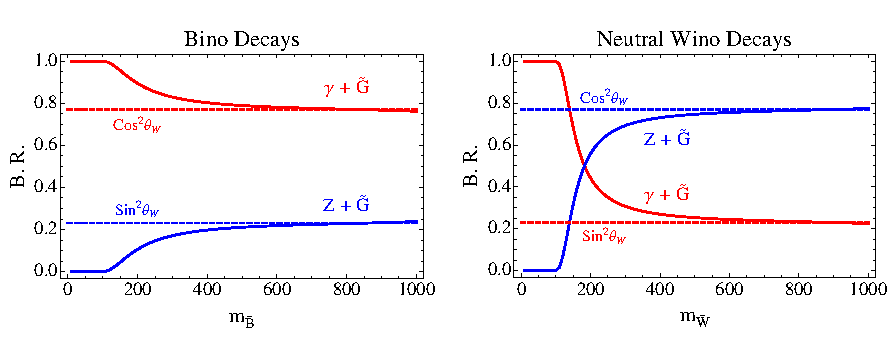
\includegraphics[width=0.8\linewidth]{../Figures/NLSPwinoBinoBR}
\caption[BR for bino and neutral wino NLSP decays]{BR for bino and neutral wino NLSP decays. Plot is taken from Ref.\cite{Ruderman:2011vv}}
\label{fig:NLSPwinoBinoBR}
\end{figure*}

\item For a \textbf{wino like} NLSP, $|M_2| < |\mu|, |M_1|$. In this case, \nuone and \chone are nearly mass degenerate and the decay modes are
\begin{center}
$\chone \rightarrow W^\pm + $\grav \\%or ($\pi^{\pm} +$ \nuone + $\grav)\\
$\nuone \rightarrow Z/\gamma + $\grav
\end{center}
The right plot in Fig.\ref{fig:NLSPwinoBinoBR} shows BR for \nuone decay as a function of wino mass \cite{Ruderman:2011vv}. These scenarios can result in signatures with lepton $+\ \gamma+\ptmiss$.

\item For a \textbf{higgsino like} NLSP, $|\mu| < M_1,M_2$ and different NLSP decay modes are preferred depending on the value of $\mu$.\\
If $\mu < 0$, then $\nuone \rightarrow \higgs/\gamma + $\grav decay is preferred.\\
If $\mu > 0$, then $\nuone \rightarrow Z/\gamma + $\grav decay dominates.\\
Models with higgsino like NLSP may result in $b\bar{b}$, coming from \higgs decay, and $\gamma+\ptmiss$ final states.
\end{itemize}

\subsection{Simplified GMSB models}
As the name suggests, various simplifications are done to the actual SUSY models and searches are designed based on the simplified model scenarios (SMS) \cite{bib-sms-1,bib-sms-2,bib-sms-3,bib-sms-4,Chatrchyan:2013sza}. There are many free parameters in the theory and as a result, there is no easy way of making a prediction in an experiment. As an example, the nature of NLSP, whether it is a bino, wino, higgsino, or a mixture of these, is not predicted by the theory and hence the signatures expected in proton-proton (p-p) collisions at the LHC is not precisely known. We make certain justifiable assumptions and explicitly state these assumptions. Another advantage in using SMS is that it is easy to re-interpret the results by taking a different SUSY model.

The scenario of a natural SUSY spectrum with GMSB and $R$-parity conservation typically manifests as events with multiple jets, at least one photon, and large \ptmiss. Depending on the topology, these jets can arise from either light-flavored quarks (\cPqu, \cPqd, \cPqs, \cPqc) or {\cPqb} quarks. We study four simplified models; example diagrams depicting these models are shown in Fig.~\ref{fig:SMS_diagram}.
Three models involve gluino pair production (prefixed with T5), and one model involves top squark pair production (prefixed with T6).
In the T5qqqqHG model, each gluino decays to a pair of light-flavored quarks (\qqbar) and a neutralino.  The T5bbbbZG and T5ttttZG models are similar to T5qqqqHG, except that the each pair of light-flavored quarks is replaced by a pair of bottom quarks (\bbbar) or a pair of top quarks (\ttbar), respectively. In the T5qqqqHG model, the \nuone decays either to an SM Higgs boson and a \grav or to a photon and a \susyP{G}.  The $\nuone\to\higgs\grav$ branching fraction is assumed to be 50\%, and the smallest \nuone mass considered is 127 \gev. In the T5bbbbZG and T5ttttZG models, the neutralinos decay to $Z\grav$ and $\gamma\grav$ with equal probability. The T6ttZG model considers top squark pair production, with each top squark decaying into a top quark and a neutralino. The neutralino can then decay with equal probability to a photon and a \grav or to a Z boson and a \grav. For the models involving the decay $\nuone\to Z\grav$, we probe \nuone masses down to 10 \gev. All decays of SUSY particles are assumed to be prompt. In all models, the mass \grav is fixed to be 1 \gev, to be consistent with other published results of CMS experiment. For the parameter space explored here, the kinematic properties do not depend strongly on the exact value of \grav.

\begin{figure*}[htb]
\centering
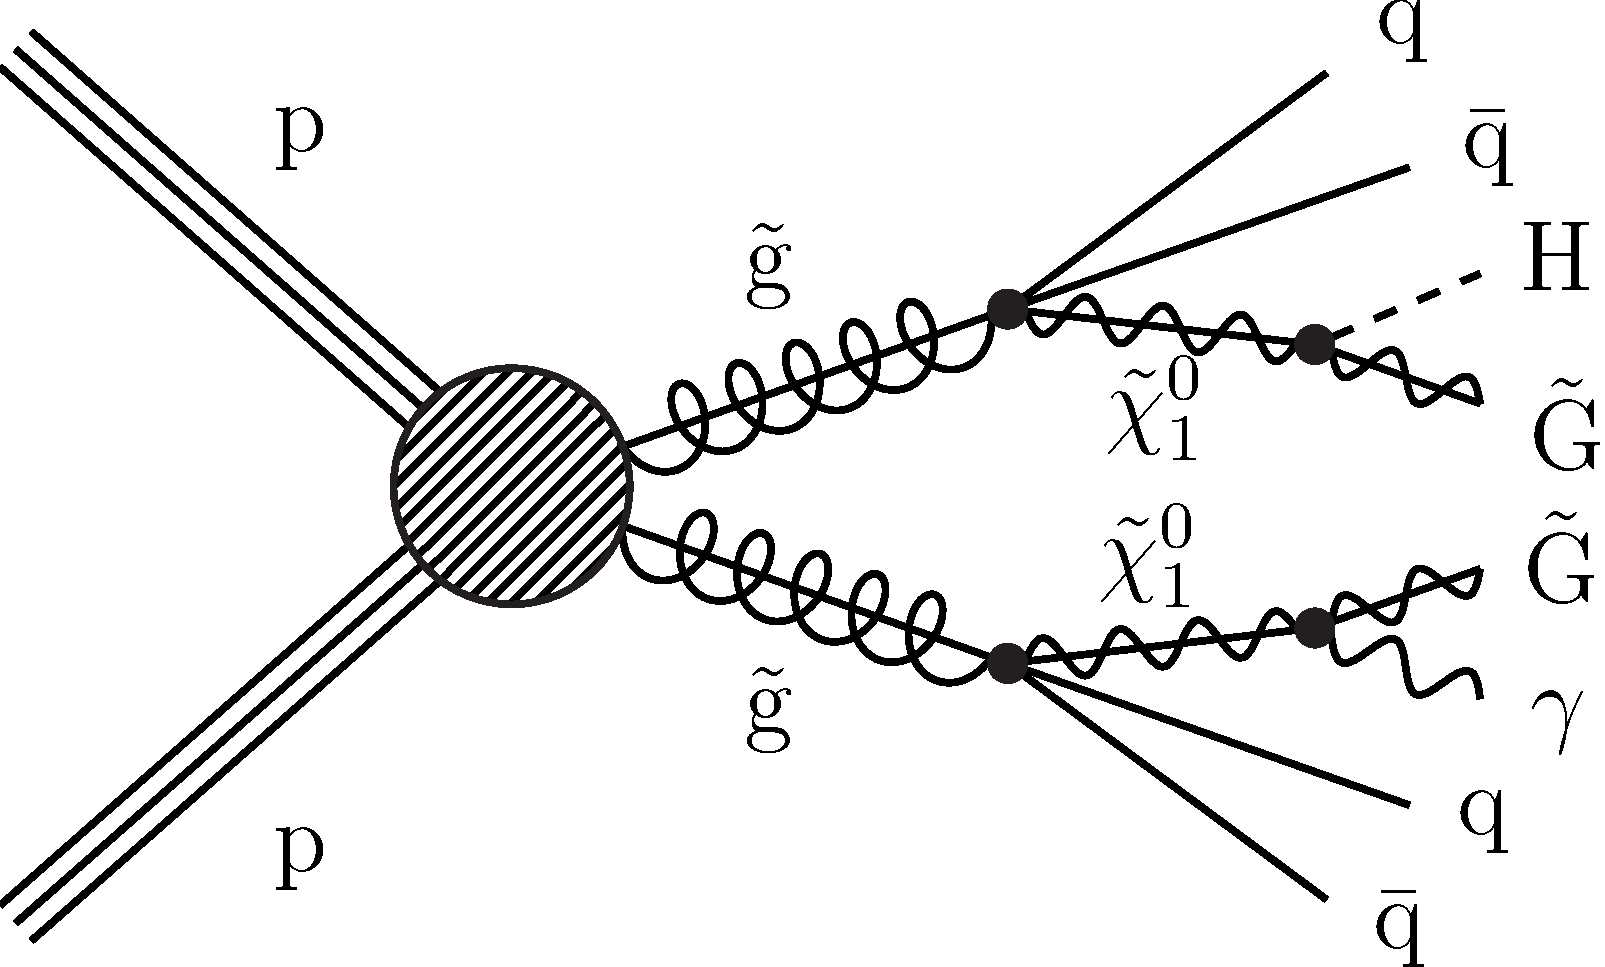
\includegraphics[width=0.4\linewidth]{../Figures/Figure_001-a.pdf}\hspace{0.05\linewidth}
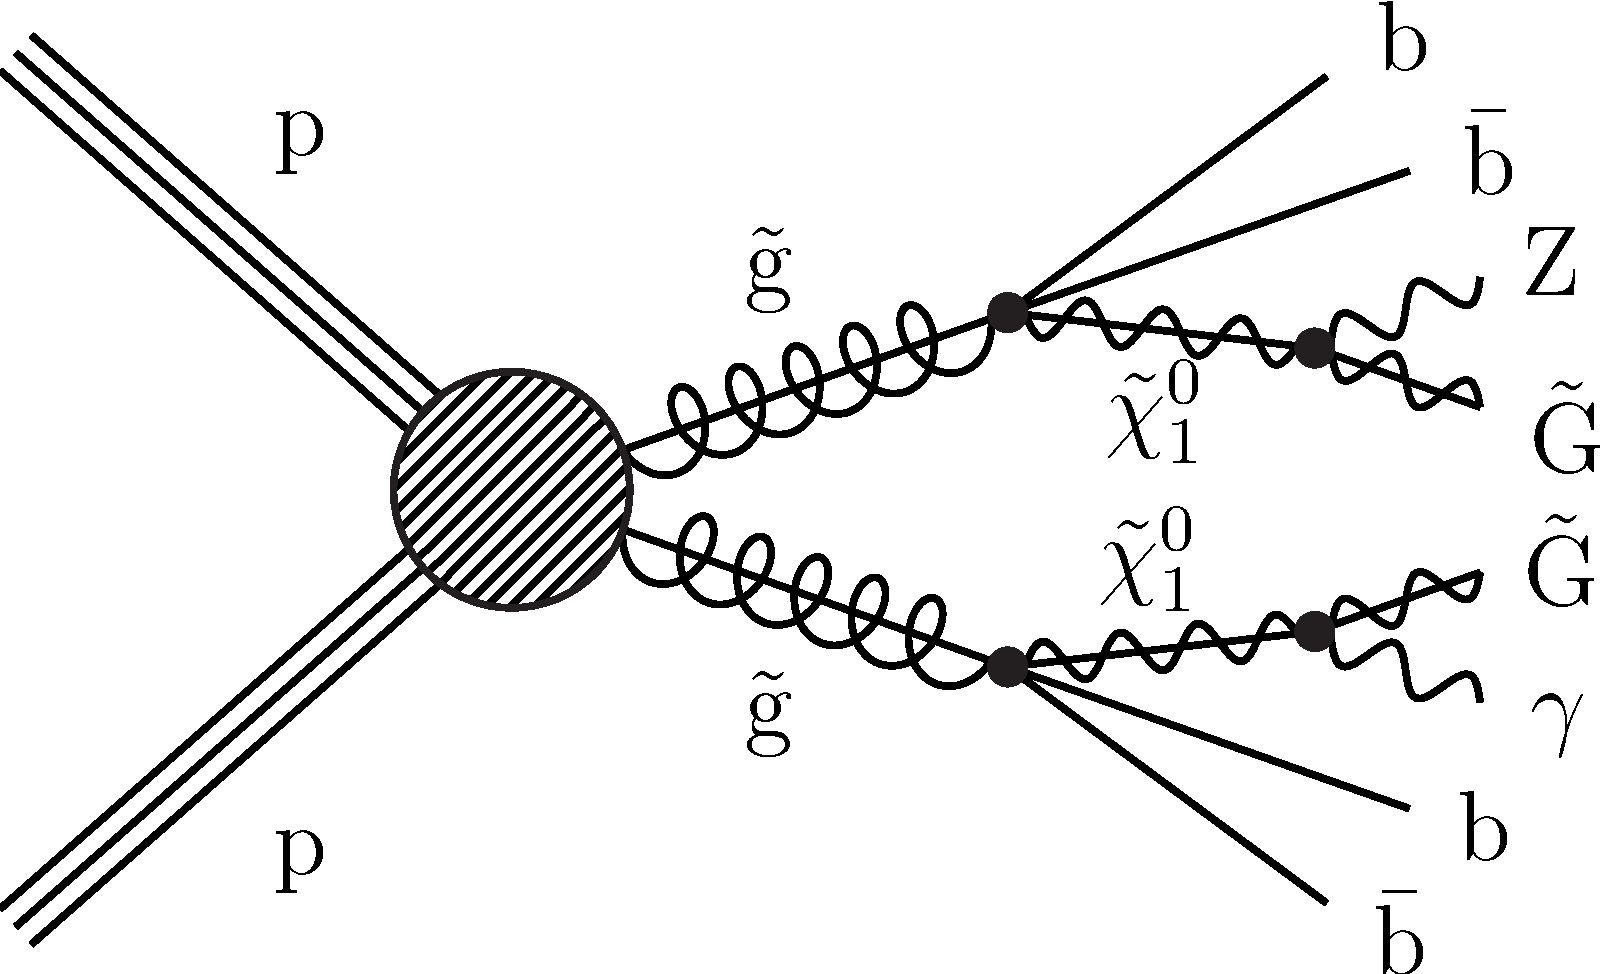
\includegraphics[width=0.4\linewidth]{../Figures/Figure_001-b.pdf}\\
\vspace{1.0cm}
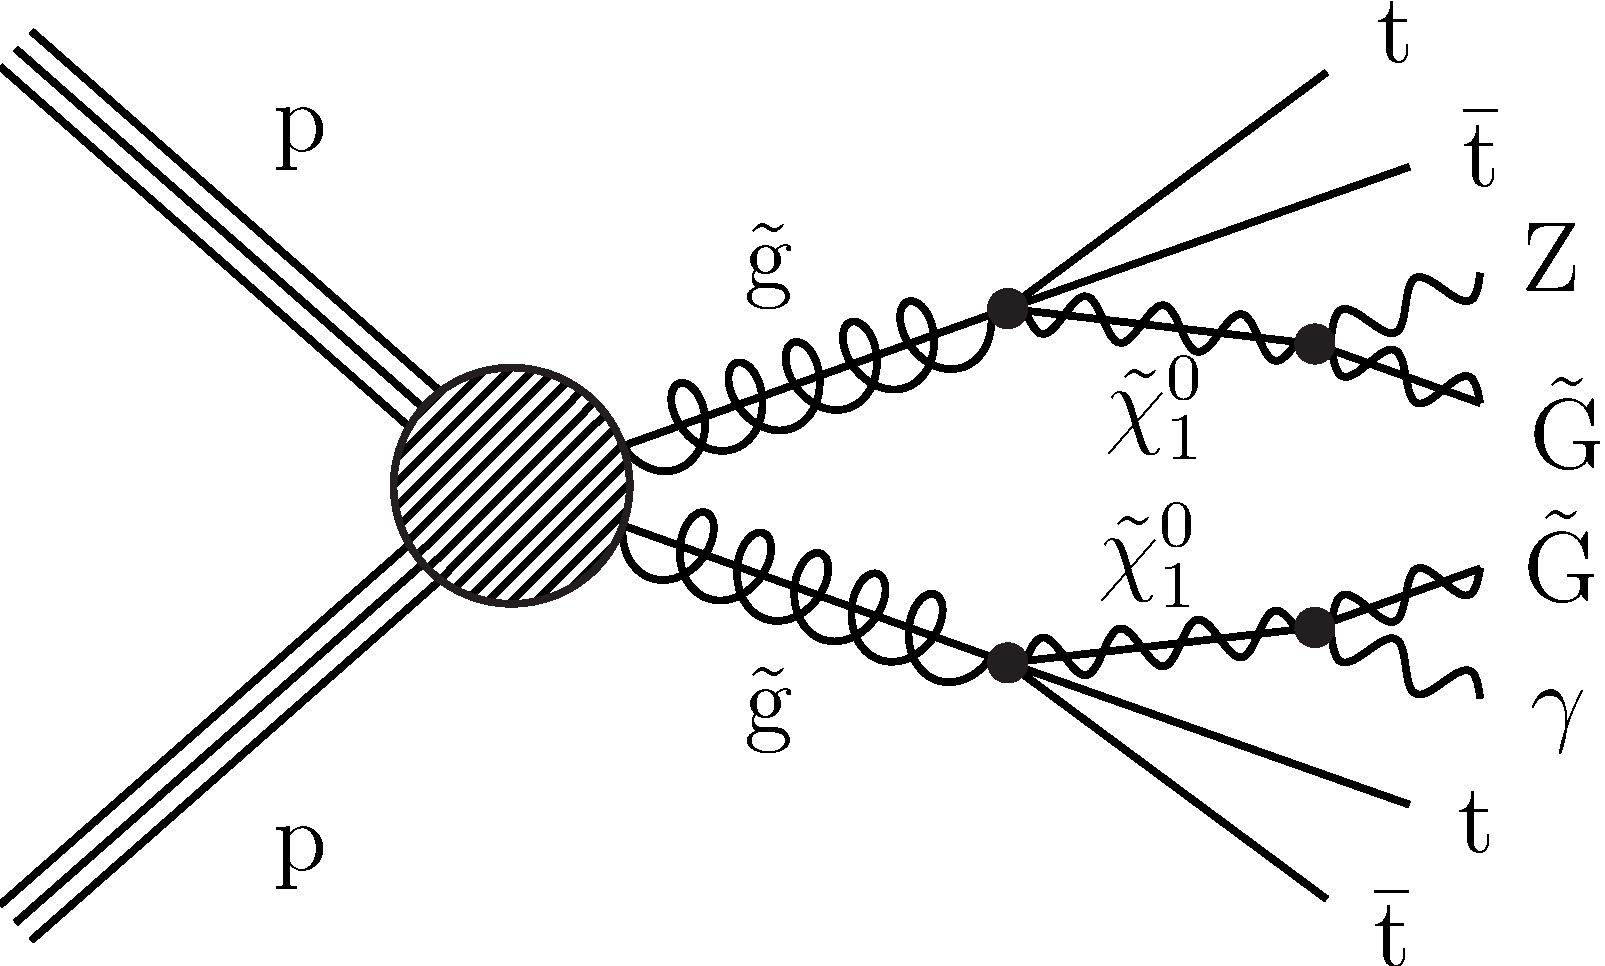
\includegraphics[width=0.4\linewidth]{../Figures/Figure_001-c.pdf}\hspace{0.05\linewidth}
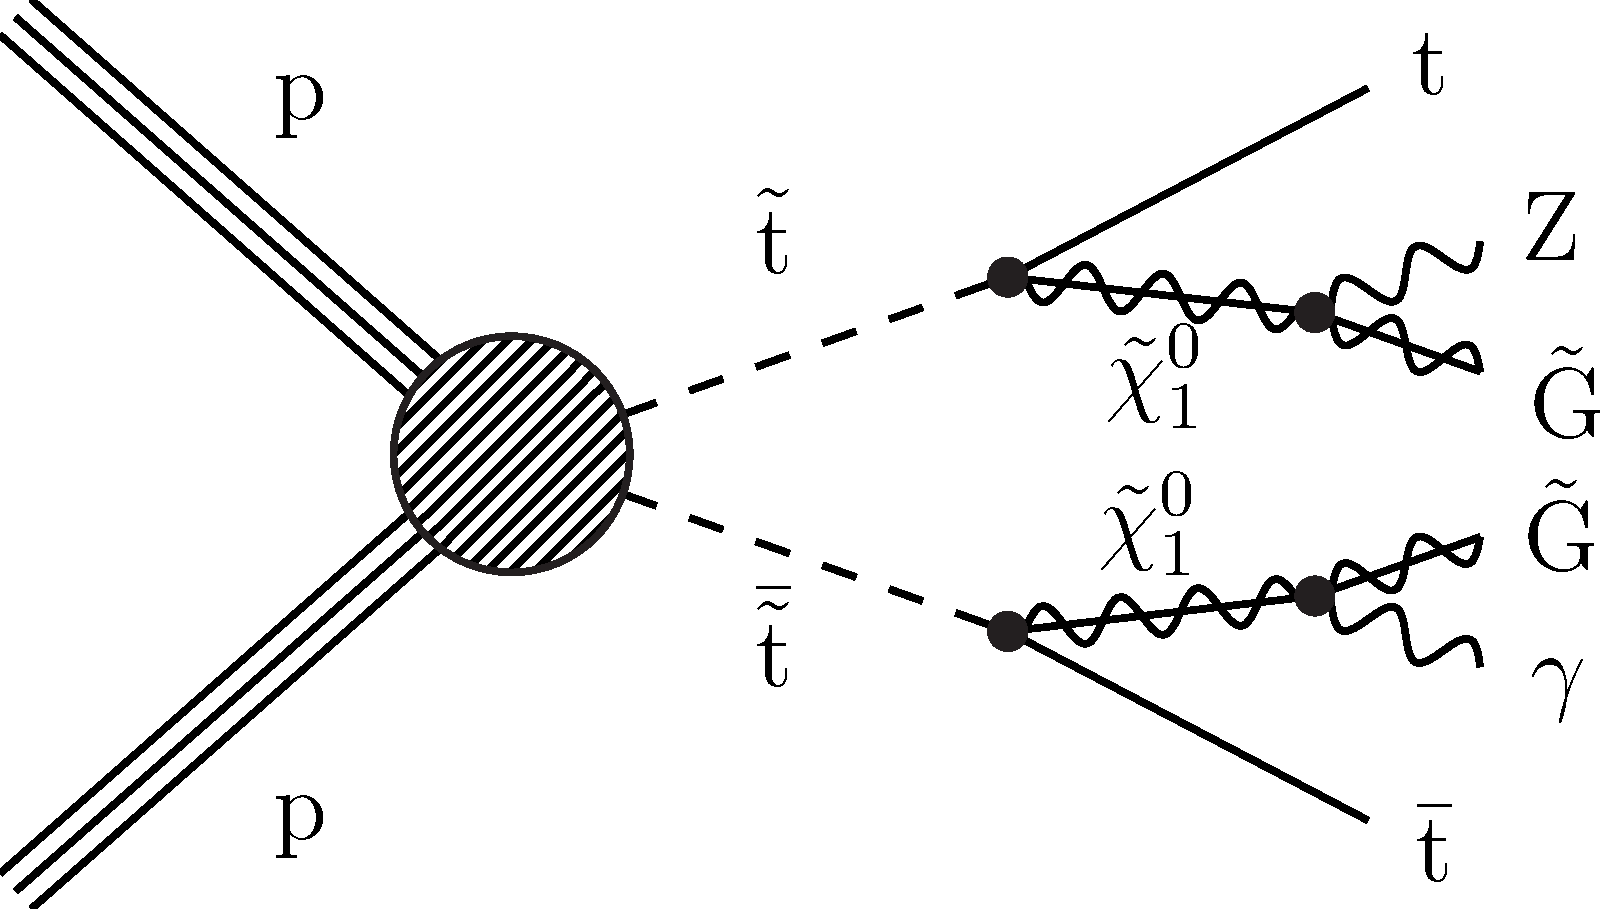
\includegraphics[width=0.4\linewidth]{../Figures/Figure_001-d.pdf}
\caption[SMS diagrams]{Example diagrams depicting the simplified models used, which are defined in the text. The top left diagram depicts the T5qqqqHG model, the top right diagram depicts the T5bbbbZG model, the bottom left diagram depicts the T5ttttZG model, and the bottom right depicts the T6ttZG model.}
\label{fig:SMS_diagram}
\end{figure*}





